% ****** Start of file apssamp.tex ******
%
%   This file is part of the APS files in the REVTeX 4.1 distribution.
%   Version 4.1r of REVTeX, August 2010
%
%   Copyright (c) 2009, 2010 The American Physical Society.
%
%   See the REVTeX 4 README file for restrictions and more information.
%
% TeX'ing this file requires that you have AMS-LaTeX 2.0 installed
% as well as the rest of the prerequisites for REVTeX 4.1
%
% See the REVTeX 4 README file
% It also requires running BibTeX. The commands are as follows:
%
%  1)  latex apssamp.tex
%  2)  bibtex apssamp
%  3)  latex apssamp.tex
%  4)  latex apssamp.tex
%
\documentclass[%
 reprint,
%superscriptaddress,
%groupedaddress,
%unsortedaddress,
%runinaddress,
%frontmatterverbose, 
%preprint,
%showpacs,preprintnumbers,
nofootinbib,
%nobibnotes,
%bibnotes,
 amsmath,amssymb,
 aps,
%pra,
%prb,
%rmp,
%prstab,
%prstper,
%floatfix,
]{revtex4-1}

\usepackage{graphicx}% Include figure files
\usepackage{dcolumn}% Align table columns on decimal point
\usepackage{bm}% bold math
\usepackage{amssymb}
\usepackage{amsmath}
\usepackage{graphicx}
\usepackage{courier}


\DeclareMathOperator*{\argmax}{arg\,max}
\DeclareMathOperator*{\argmin}{arg\,min}

\newcommand{\abs}[1]{\left\|{#1}\right\|}

%\usepackage{hyperref}% add hypertext capabilities
%\usepackage[mathlines]{lineno}% Enable numbering of text and display math
%\linenumbers\relax % Commence numbering lines

%\usepackage[showframe,%Uncomment any one of the following lines to test 
%%scale=0.7, marginratio={1:1, 2:3}, ignoreall,% default settings
%%text={7in,10in},centering,
%%margin=1.5in,
%%total={6.5in,8.75in}, top=1.2in, left=0.9in, includefoot,
%%height=10in,a5paper,hmargin={3cm,0.8in},
%]{geometry}

\begin{document}

%\preprint{APS/123-QED}

\title{Improving the Q Learning Algorithm with Rudimentary AI}% Force line breaks with \\
%\thanks{A footnote to the article title}%

\author{Burke Brockelbank}

\date{\today}% It is always \today, today,
             %  but any date may be explicitly specified

\begin{abstract}
Neural networks have effectively been taught to play video games. These neural nets have historically been trained through a method of reinforcement learning called Q learning. One of the major challenges with this method occurs in the early stages of training when the quality function is most inaccurate. Here we show a method for skipping past this initial training phase, decreasing the time to convergence. In this method, the neural net first trains on labelled data generated by a sub-optimal, but theoretically simple, artificial intelligence until it is capable of playing the game to a similar effectiveness. It is then trained with Q learning to refine the performance of the AI. This method is applicable to any Q learning scenario where it is easy to concieve an AI to prepare labelled data.
\end{abstract}

\maketitle

%\tableofcontents

\section{\label{sec:Introduction}Introduction}
The method of training explored in this report is Q learning. Q learning has always had the problem of slow convergence near the beginning of its training, an issue that is inherent its formulation. Q learning is shown to theoretically converge in infinite time with some restrictions on the learning rate in \cite{sutton1998reinforcement} and has proven capable of converging with no assistance in practice, however the amount of computation power and time needed to do this may not always be feasible. Additionally, it is better to avoid the problems with Q learning rather than trust in the theory in case a specific implementation makes it impossible to use.

Another issue with reinforcement learning is that its behavior is highly dependent on how the reward function is specified. Poor choices of reward functions can lead the model to make decisions which are not desired. In \cite{clark_amodei_2017} the authors describe an interesting example where the specific reward function they used lead to a difference between how they wanted their player to act and how their player ended up maximizing reward.

\subsection{\label{sec:QualityFunction}The Quality Function}
 The formulation of DQ begins with specifying the reward of an action. Suppose that there is a player in a state $s$ who takes an action $a$. This action will move the player from the state $s$ to $s'$ and also give the player some immediate reward $r(s,a)$. For example, if the player is a robo-advisor that is trading stocks then the state is the current price of all stocks and the action is either to wait, sell a stock, or buy a stock. The reward may be specified as the amount of value gained in moving from the state $s$ to $s'$. After this the player will take the action $a'$ from the state $s'$, followed by taking the action $a''$ from the consequent state $s''$ and so on. The cumulative reward $R$ will include all of these rewards, but to reflect the uncertainty about future actions, a discount factor $\gamma\in(0,1)$ is introduced.
\begin{equation}
  R =  r_{s,a} + \gamma r_{s',a'} + \gamma^2 r_{s'',a''} + \hdots, \label{eq:CumulativeReward}
\end{equation}
Suppose we had some ideal policy function $\pi^*$ that we could consult at every step to give us the ideal action to maximize total reward given a state. Then we define our quality function as,
\begin{equation}
  Q^*(s,a) = r_{s,a} + \gamma r_{s',\pi^*(s')} + \gamma^2 r_{s'',\pi^*(s'')} + \hdots. \label{eq:Bellman1}
\end{equation}
Thus, $Q(s,a)$ represents the maximal cumulative reward we can get from the state $s$ given that we are going to perform the action $a$ from that state. We can rewrite this as,
\begin{equation}
  Q^*(s,a) = r_{s,a} + \gamma Q^*(s', \pi^*(s')). \label{eq:Bellman2}
\end{equation}
which is known as the Bellman equation. Additionally, $\pi^*$ can then be written in terms of $Q^*$ as,
\begin{equation}
  \pi^*(s) = \argmax_a Q^*(s,a). \label{eq:Policy1}
\end{equation}

The objective of Q learning is to use a neural net to model this quality function. Let the approximation be $Q$. Define a policy function analogously to \eqref{eq:Policy1},
\begin{equation}
  \pi(s) = \argmax_a Q(s,a). \label{eq:Policy2}
\end{equation}

 Then there will be some difference between the two sides of \eqref{eq:Bellman2} called $\delta$.
\begin{equation}
  Q(s,a) = r_{s,a} + \gamma Q(s', \pi(s')) + \delta. \label{eq:delta}
\end{equation}
The loss is then calculated as a function of $\delta$.

In order to train the neural net effectively, some degree of exploration is used. In the case of this report, $\pi$ is replaced with $\pi_\epsilon$ where $\epsilon\in[0,1]$. $\pi_\epsilon$ has a probability $\epsilon$ of returning a random action and a $(1-\epsilon)$ probability of returning $\pi$. 

\subsection{\label{sec:Monkey}Monkey Want Banana}
This report considers the performance of a neural net playing a simple game where the player controls a monkey in a square grid trying to collect bananas while traversing walls and avoiding lava. Every action the monkey takes expends some of its food so it must constantly find new bananas to eat. The game is written with a text-based ASCII art interface. One screen of the game is shown in Figure \ref{fig:GameDemo}.

\begin{figure}
  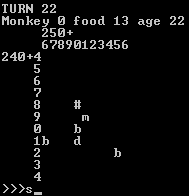
\includegraphics[width=0.8\columnwidth]{GameDemo}
  \caption{A demonstration of the monkey game showing all the block types and the movement interface. Block types are barriers \texttt{\#}, monkeys \texttt{m}, bananas \texttt{b}, and lava \texttt{d} which is symbolized by a \texttt{d} for danger. The line beginning with \texttt{>>>} is the movement interface. In this case, the player has chosen to move downwards. These controls are defined with the common \texttt{wasd} movements. Additionally the player can choose not to move by entering a space key which we will symbolize as \texttt{\_}. The numbers on the perimeter of the map show the position of objects on the map by splitting it into a number modulo 10 and the ones digit. In this image, the monkey is at position (239,251).} \label{fig:GameDemo}
\end{figure}

A natural choice of reward function is the food level. Specifically, the immediate reward of some action $a$ taking the game state from $s$ to $s'$ is the food level in $s'$ minus the food level in $s$. Doing an action takes one food away from the monkey, so if no banana is eaten, the immediate reward is $-1$. Eating a banana give the monkey 5 food, so if the monkey moves to collect a banana, it gets an immediate reward of $4$. The monkey also may starve to death, or move into lava, in which case it will get a reward of $-50$. The discount factor was set to $0.8$ since this fairly accurately describes the lack of knowlege the monkey has outside of its $11x11$ vision range.

The loss function was decided as the smooth L1 loss,

\begin{equation}
  \text{loss}(\delta) = \left\{ \begin{array}{cc} \frac{1}{2} \delta^2 & \abs{\delta} \leq 1 \\ \abs{\delta} - \frac{1}{2} & \abs{\delta} > 1\end{array}. \right. \label{eq:Loss}
\end{equation}

\subsection{\label{sec:Challenges}Challenges with Q Learning}
One of the main issues with Q learning is evident in \eqref{eq:delta}. Calculating the loss for performing the action $a$ from the state $s$, it depends on the next state. Hypothetically, $\delta$ could be very small or even zero even if $Q$ does not accurately model $Q^*$ as long as $Q(s,a)$ and $\gamma Q(s', \pi(s'))$ differ from their respective $Q^*$ predictions by the same amount. If $Q$ is inaccurate, like at the beginning of its training, it will converge slowly.

For an example of this challenge in the monkey game, consider the series of states in Figure \ref{fig:States}. First we will derive $Q^* $ from the states in Figure \ref{fig:States} and then show how with some issues in $Q$ can cause slow learning. We can work backwards from the final state to derive $Q^*$. Assuming that after $s'''$ the monkey cannot find any more bananas and does not die, it will just eat one food per turn and thus have each immediate reward be $-1$. The quality can be determined via \eqref{eq:Bellman1} as,

\begin{equation}
  Q^*(s''',a''') = (-1) + \gamma (-1) + \gamma^2 (-1) + \hdots = -5.
\end{equation}

From this we calculate all previous qualities via \eqref{eq:Bellman2}.

\begin{align}
  Q^*(s'',a'') &= (-1) + \gamma Q^*(s''',a''') = -5,\\
  Q^*(s',a') &= (4) + \gamma Q^*(s'',a'') = 0,\\
  Q^*(s,a) &= (-1) + \gamma Q^*(s',a') = -1.
\end{align}

Suppose that $Q$ misevaluates $Q(s'',a'')$ as 0 and $Q(s',a')$ as $4$. Then \eqref{eq:delta} becomes,
\begin{align*}
  Q(s',a') &= r_{s,a} + \gamma Q(s'', \pi(s'')) + \delta \\
  4 &= 4 + \gamma 0 + \delta \\
  \delta &= 0.
\end{align*}

This gives a loss of zero so no learning will be done from the evaluation from state $s'$ until $Q(s'',a'')$ changes. This same effect occurs during training with the effect of making delta either too large or too small. This arises from the fact that, at the beginning of training, $Q$ does not come close to satisfying the Bellman equation. However, if $Q$ is already close to $Q^*$ then it will be close to the Bellman equation and the effect will not be as pronounced.

%\begin{figure}
%  \begin{tabular}{c|c|c}
%    &&\texttt{b}\\ \hline
%    &\texttt{\hphantom{m}}&\\ \hline
%    \texttt{m}&&
%  \end{tabular}
%  $\xrightarrow[s \quad s']{a}$
%  \begin{tabular}{c|c|c}
%    &&\texttt{b}\\ \hline
%    \texttt{\hphantom{m}}&&\\ \hline
%    &\texttt{m}&
%  \end{tabular}
%  $\xrightarrow[s' \quad s'']{a}$
%  \begin{tabular}{c|c|c}
%    &&\texttt{b}\\ \hline
%    &\texttt{m}&\\ \hline
%    \texttt{\hphantom{m}}&&
%  \end{tabular}
%  $\xrightarrow[s^{(3)} \quad s^{(4)}]{a^{(3)}}$\\
%  \begin{tabular}{c|c|c}
%    \texttt{\hphantom{m}}&&\texttt{b}\\ \hline
%    &&\texttt{m}\\ \hline
%    &\texttt{\hphantom{m}}&
%  \end{tabular}
%  $\xrightarrow[s^{(4)} \quad s^{(5)}]{a^{(4)}}$
%  \begin{tabular}{c|c|c}
%    \texttt{\hphantom{m}}&&\texttt{m}\\ \hline
%    && \\ \hline
%    &\texttt{\hphantom{m}}&
%  \end{tabular}
%  $\xrightarrow[s^{(5)} \quad s^{(6)}]{a^{(5)}}$
%  $\hdots$
%  \caption{A series of hypothetical states in the monkey game. The actions taken in this series represent one of the possible sets of actions that would be given by consulting $\pi^*$ at every state.} \label{fig:States}
%\end{figure}


\begin{figure}
  \begin{tabular}{|c|c|}
    \hline
    &\texttt{b}\\ \hline
    \texttt{m}&\\\hline
  \end{tabular}
  $\xrightarrow[s \quad s']{a}$
  \begin{tabular}{|c|c|}
    \hline
    &\texttt{b}\\ \hline
    \texttt{\hphantom{m}}&\texttt{m}\\\hline
  \end{tabular}
  $\xrightarrow[s' \quad s'']{a}$
  \begin{tabular}{|c|c|}
    \hline
    &\texttt{m}\\ \hline
    \texttt{\hphantom{m}}&\\\hline
  \end{tabular}
  $\xrightarrow[s'' \quad s''']{a''}$
  $\hdots$
  \caption{A series of hypothetical states in the monkey game. The actions taken in this series represent one of the possible sets of actions that would be given by consulting $\pi^*$ at every state.} \label{fig:States}
\end{figure}


\section{\label{sec:Methods}Methods}

The training of the neural net came in three major forms. In the first form, the neural net was trained on labelled data generated by the AI. In the second form, the neural net was trained in some curated situations to fix some deficiencies likely caused by issues in the labelled data. This form will be called curated training. Different levels of curated training are shown in Figure \ref{fig:Curation}. In the third form, the neural net was allowed to explore and learn on its own in the same environment that the AI ran in. This form will be called random reinforcement training

\begin{figure}
  \begin{tabular}{|c|c|c|}
    \hline
    &\texttt{b}&\\ \hline
    \texttt{b}&\texttt{m}&\texttt{b}\\ \hline
    &\texttt{b}& \\ \hline
  \end{tabular}\quad
  \begin{tabular}{|c|c|c|}
    \hline
    \texttt{b}&\texttt{b}&\texttt{b}\\ \hline
    \texttt{b}&\texttt{m}&\texttt{b}\\ \hline
    \texttt{b}&\texttt{b}&\texttt{b} \\ \hline
  \end{tabular}\quad
  \begin{tabular}{|c|c|c|c|c|}
    \hline
    \texttt{b}&\texttt{b}&\texttt{b}&\texttt{b}&\texttt{b}\\ \hline
    \texttt{b}&&&&\texttt{b}\\ \hline
    \texttt{b}&&\texttt{m}&&\texttt{b}\\ \hline
    \texttt{b}&&&&\texttt{b}\\ \hline
    \texttt{b}&\texttt{b}&\texttt{b}&\texttt{b}&\texttt{b}\\ \hline
  \end{tabular} \\
\caption{Levels 0, 1, and 2 or curated training are illustrated. Places where bananas are allowed to be placed are marked with a \texttt{b} while the monkey's position is marked with an \texttt{m}. Only one banana is placed in any instance of curaten training.} \label{fig:Curation}
\end{figure}

In the first part of training labelled data had to be created for the AI to play in. Data was created in game boards which had monkeys, bananas, and lava but no barriers. It was determined that adding in barriers caused the AI to get stuck far too often so data was generated without them. Even without barriers, the AI often got stuck in infinite loops which added noise to the dataset. Another source of noise is that the monkey's position was periodically reset in order to avoid stalling permanently when stuck. These are likely the reason that the model didn't converge well on the AI and was incapable of replicating it. Despite this, the first phase of training proved invaluable to the overall training. When we attempted to skip this step, the model could not be trained to effectively retrieve bananas in a reasonable amount of time.

The second part of training was meant to address some obvious shortcomings that came from training on such a poor data set. This part included both curated training and random reinforcement. Initially, the model underwent curated training of level 0, then level 1, then level 0 again. This part of the training may not have been necessary as the monkey was correctly moving towards the The model trained with the Q learning algorithm on successive stages of putting a banana close to the monkey at increasing distance at each stage. These stages ran until the monkey could consistently approach bananas up to a distance of two blocks away.



\section{\label{sec:Results}Results}

The model was then tested against the AI in a room with a random distribution of 2\% barriers, 1\% lava, and 5\% bananas

emphasize how the AI was so simple and really insufficient for the task at hand but was necessary in creating a much more effective neural net

\section{\label{sec:Discussion}Discussion}

talk about how the convolutional branch of the neural net was not sufficient for dealing with far-away objects alone and the neural net would likely benefit breatly by expanding the non-convolutional branch out to the full 11x11 grid.

\bibliographystyle{apsrev4-1}
\bibliography{bib}

\end{document}
%
% ****** End of file apssamp.tex ******



























